\chapter{\color{red} 界面设计}
%==============================================================
    \section{客户端界面}
    \begin{figure}[h]
        \centering
        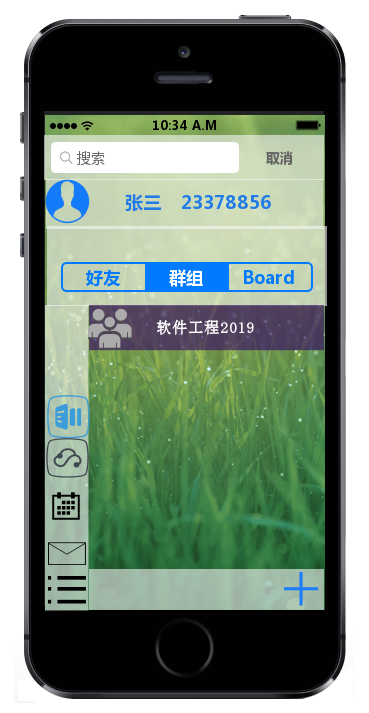
\includegraphics[scale=0.6]{OutlineDesign/figures/客户端界面.png}
        \caption{客户端界面}
        \label{fig:server_flow}
        \note{左下快捷方式从上到下依次为:在线文档协作,云文件管理,日历,邮箱,菜单栏,右下为添加新的好友/群聊}
    \end{figure}
    \newpage
    %--------------------------------------------------------------------------
    \section{服务器端界面}
    %=================================
    % 此处应当有一个简略的图。
    %=================================
    \begin{figure}[h]
        \centering
        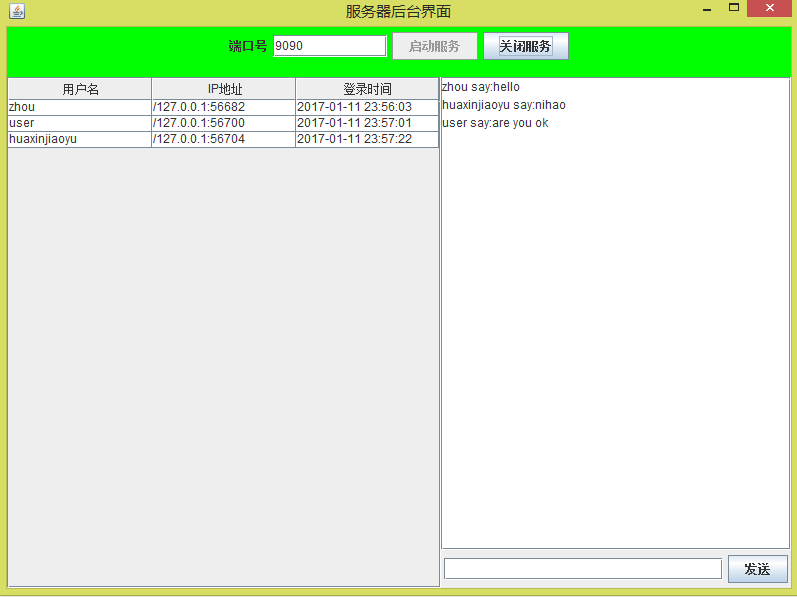
\includegraphics[scale=0.7]{OutlineDesign/figures/服务器端界面.png}
        \caption{服务器端界面}
        \label{fig:server_flow}
    \end{figure}
    \newpage
    %--------------------------------------------------------------------------
    \section{登录界面}
    %=================================
    % 此处应当有一个简略的图。
    %=================================
    \begin{figure}[h]
        \centering
        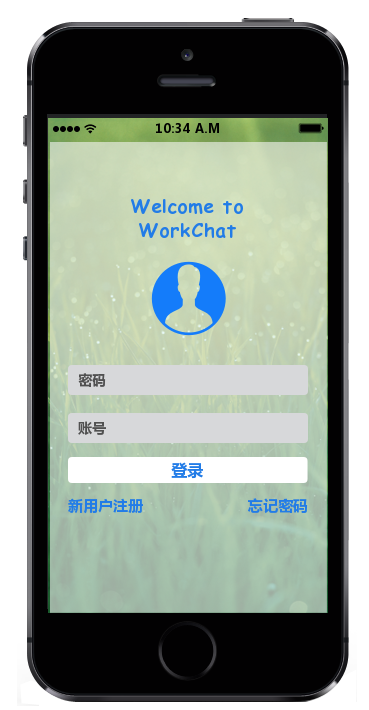
\includegraphics[scale=0.7]{OutlineDesign/figures/登录界面.png}
        \caption{登录界面}
        \label{fig:server_flow}
    \end{figure}
    \newpage
    %--------------------------------------------------------------------------
    \section{R.INTF.CALC.001:一对一即时通讯功能界面}
    %=================================
    % 此处应当有一个简略的图。
    %=================================
    \begin{figure}[h]
        \centering
        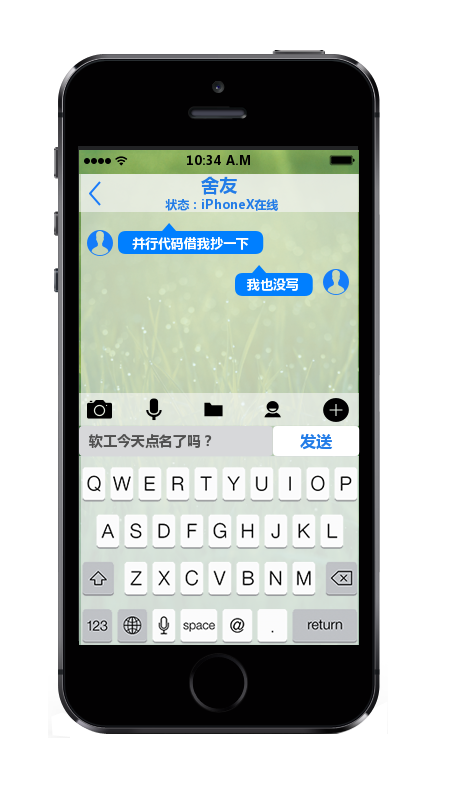
\includegraphics[scale=0.6]{OutlineDesign/figures/一对一即时通讯功能界面.png}
        \caption{一对一即时通讯功能界面}
        \label{fig:server_flow}
    \end{figure}
    \newpage
    %--------------------------------------------------------------------------
    \section{R.INTF.CALC.002.1: 群管理功能界面}
    \begin{figure}[h]
        \centering
        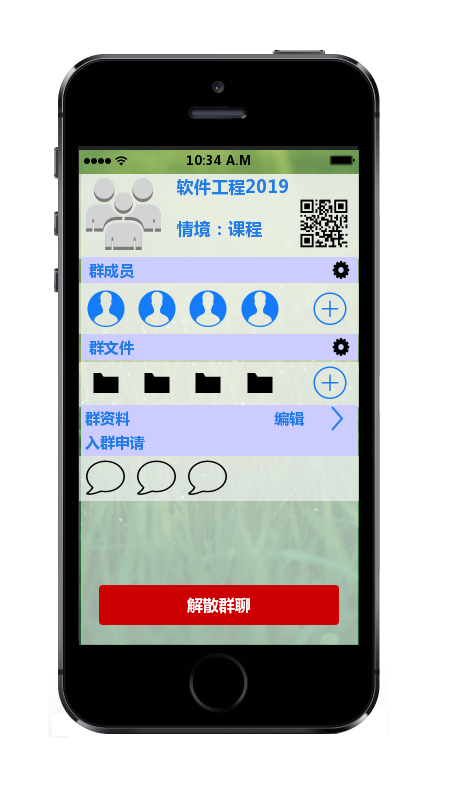
\includegraphics[scale=0.6]{OutlineDesign/figures/群管理功能界面.png}
        \caption{群管理功能界面}
        \label{fig:server_flow}
    \end{figure}
    \newpage
    %--------------------------------------------------------------------------
    \section{R.INTF.CALC.002.2: 群聊天功能界面}
    \begin{figure}[h]
        \centering
        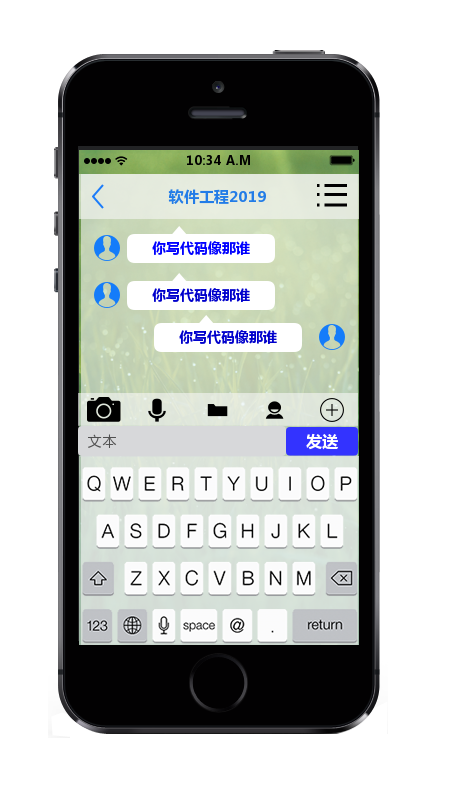
\includegraphics[scale=0.6]{OutlineDesign/figures/群聊天功能界面.png}
        \caption{群聊天功能界面}
        \label{fig:server_flow}
    \end{figure}
    \newpage
    %--------------------------------------------------------------------------
    \section{R.INTF.CALC.002.3: 情境功能界面}
    \begin{figure}[h]
        \centering
        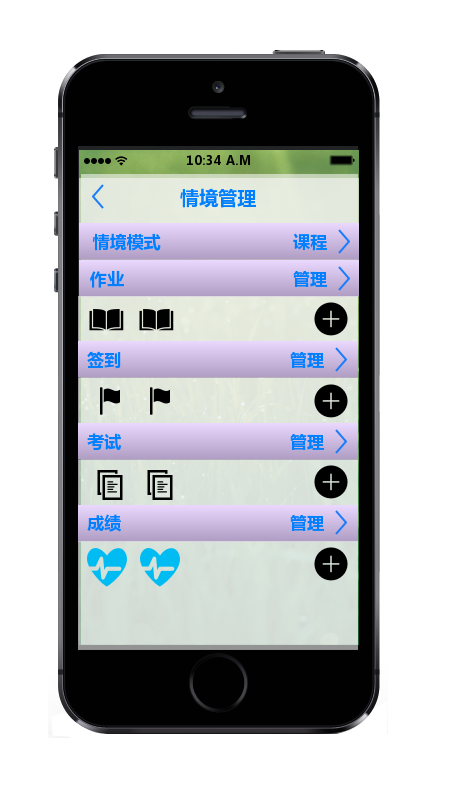
\includegraphics[scale=0.6]{OutlineDesign/figures/情境功能界面.png}
        \caption{情境功能界面}
        \label{fig:server_flow}
    \end{figure}
    \newpage
    %--------------------------------------------------------------------------
    \section{\color{red}R.INTF.CALC.002.4: 问题功能}
    \begin{figure}[h]
        \centering
        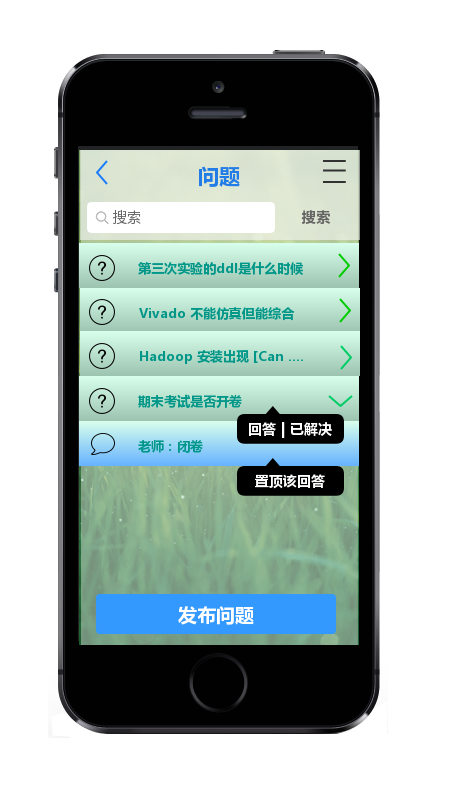
\includegraphics[scale=0.6]{OutlineDesign/figures/问题功能功能界面.png}
        \caption{\color{red}问题功能功能界面}
        \label{fig:server_flow}
    \end{figure}
    \newpage
    %--------------------------------------------------------------------------
    \section{R.INTF.CALC.003: 活动/任务发布与管理功能界面}
    \begin{figure}[h]
        \centering
        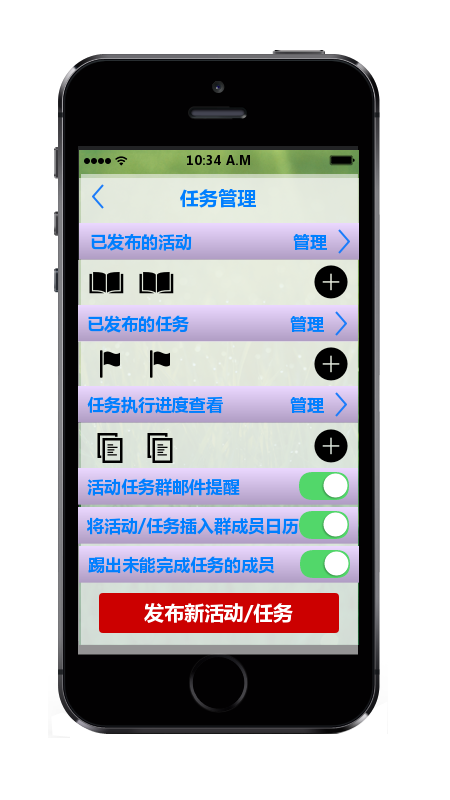
\includegraphics[scale=0.6]{OutlineDesign/figures/活动任务发布与管理功能界面.png}
        \caption{活动任务发布与管理功能界面}
        \label{fig:server_flow}
    \end{figure}
    \newpage
    %--------------------------------------------------------------------------
    \section{R.INTF.CALC.004: 音视频通话 (会议) 功能界面}
    \begin{figure}[h]
        \centering
        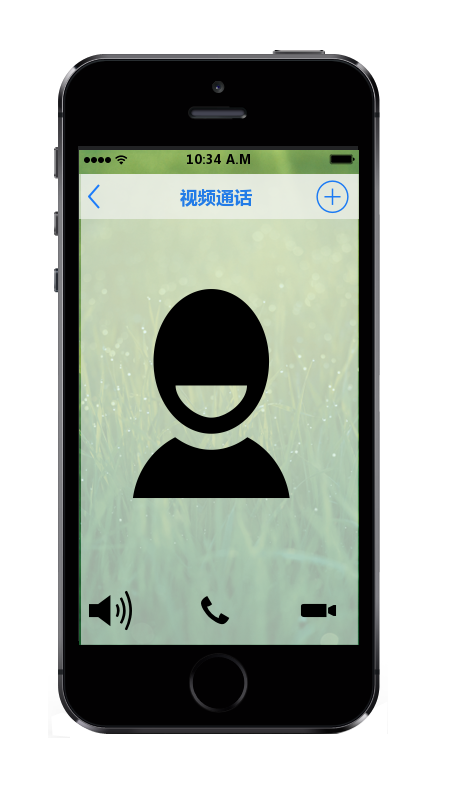
\includegraphics[scale=0.6]{OutlineDesign/figures/音视频通话会议功能界面.png}
        \caption{音视频通话 (会议) 功能界面}
        \label{fig:server_flow}
    \end{figure}
    \newpage
    %--------------------------------------------------------------------------
    \section{R.INTF.CALC.005.1: 好友管理功能界面}
    \begin{figure}[h]
        \centering
        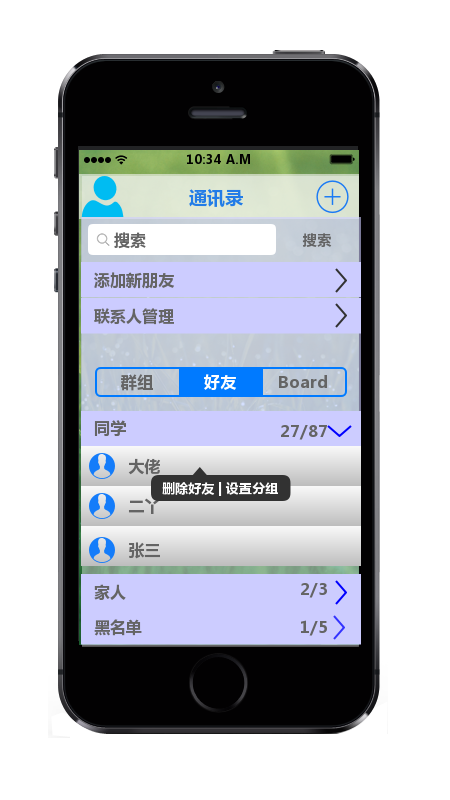
\includegraphics[scale=0.6]{OutlineDesign/figures/好友管理功能界面.png}
        \caption{好友管理功能界面}
        \label{fig:server_flow}
    \end{figure}
    \newpage
    %--------------------------------------------------------------------------
    \section{R.INTF.CALC.005.2: 群聊管理功能界面}
    \begin{figure}[h]
        \centering
        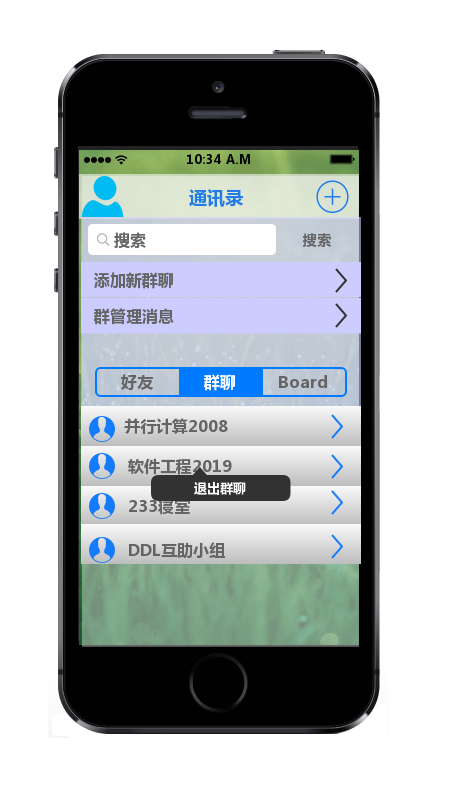
\includegraphics[scale=0.6]{OutlineDesign/figures/群聊管理功能界面.png}
        \caption{群聊管理功能界面}
        \label{fig:server_flow}
    \end{figure}
    \newpage
    %--------------------------------------------------------------------------
    \section{R.INTF.CALC.005.3: 黑名单功能界面}
    \begin{figure}[h]
        \centering
        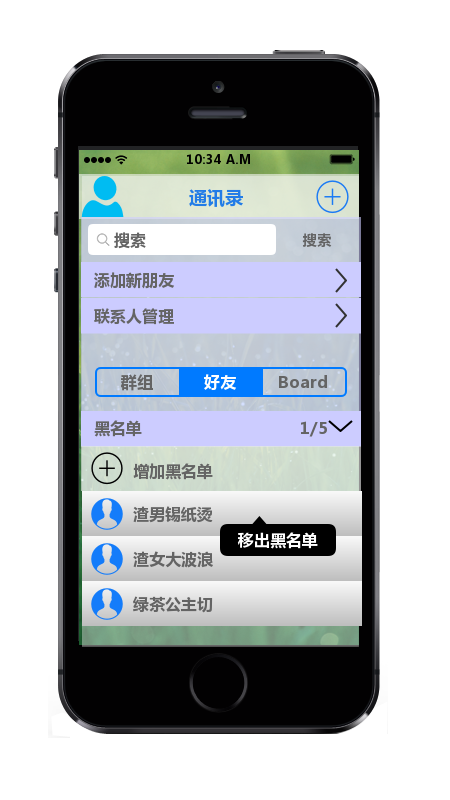
\includegraphics[scale=0.6]{OutlineDesign/figures/黑名单功能界面.png}
        \caption{黑名单功能界面}
        \label{fig:server_flow}
    \end{figure}
    \newpage
    %--------------------------------------------------------------------------
    \section{R.INTF.CALC.006: 聊天记录功能界面}
    \begin{figure}[h]
        \centering
        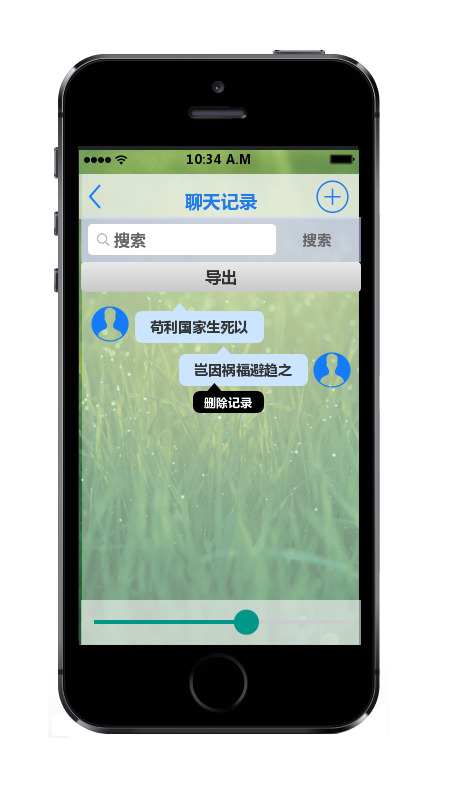
\includegraphics[scale=0.6]{OutlineDesign/figures/聊天记录功能界面.png}
        \caption{聊天记录功能界面}
        \label{fig:server_flow}
    \end{figure}
    \newpage
    %--------------------------------------------------------------------------
    \section{R.INTF.CALC.007: 消息提醒功能界面}
    \begin{figure}[h]
        \centering
        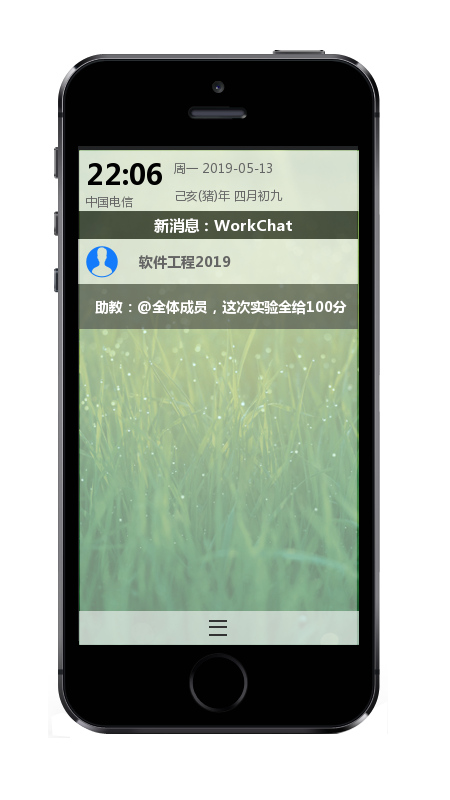
\includegraphics[scale=0.6]{OutlineDesign/figures/消息提醒功能界面.png}
        \caption{消息提醒功能界面}
        \label{fig:server_flow}
    \end{figure}
    \newpage
    %--------------------------------------------------------------------------
    \section{R.INTF.CALC.008: Board(广场) 功能界面}
    \begin{figure}[h]
        \centering
        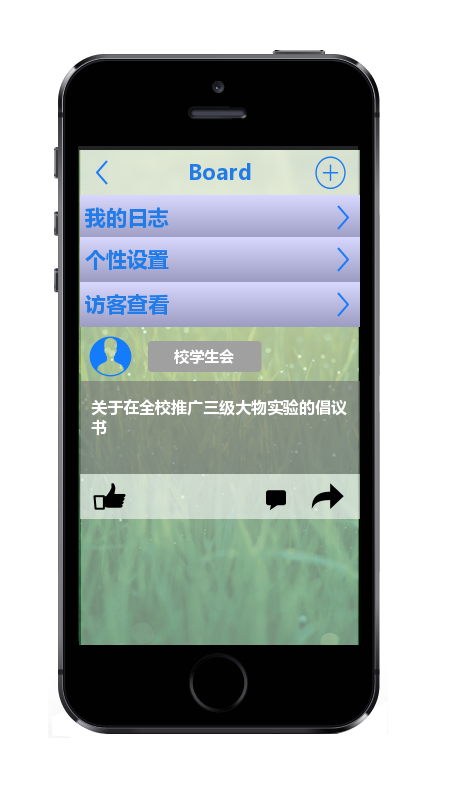
\includegraphics[scale=0.6]{OutlineDesign/figures/Board广场功能界面.png}
        \caption{Board(广场) 功能界面}
        \label{fig:server_flow}
    \end{figure}
    \newpage
    %--------------------------------------------------------------------------
    \section{R.INTF.CALC.009: 个性化好友推荐功能界面}
    \begin{figure}[h]
        \centering
        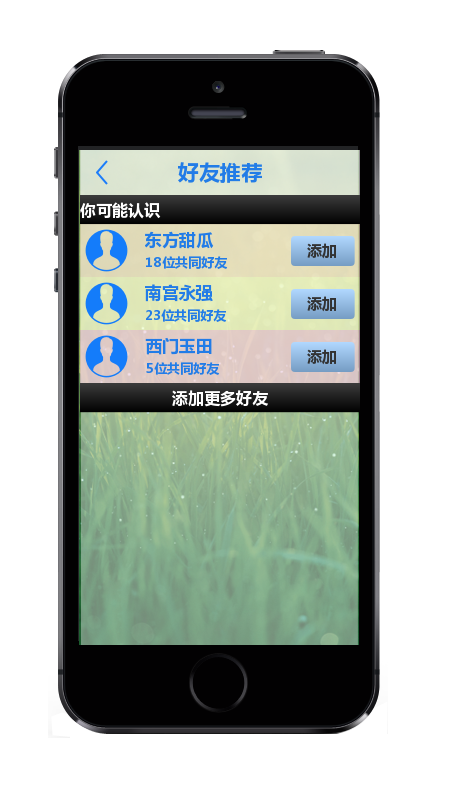
\includegraphics[scale=0.6]{OutlineDesign/figures/个性化好友推荐功能界面.png}
        \caption{个性化好友推荐功能界面}
        \label{fig:server_flow}
    \end{figure}
    \newpage
    %--------------------------------------------------------------------------
    \section{R.INTF.CALC.010: 在线文档协作平台功能界面}
    \begin{figure}[h]
        \centering
        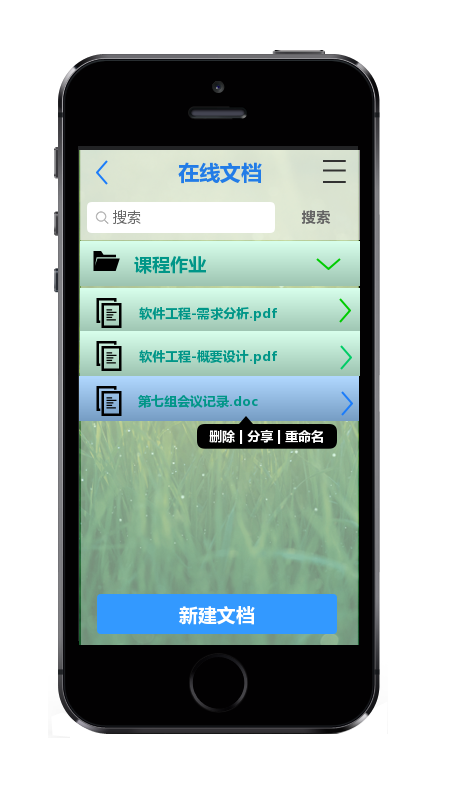
\includegraphics[scale=0.6]{OutlineDesign/figures/在线文档协作平台功能界面.png}
        \caption{在线文档协作平台功能界面}
        \label{fig:server_flow}
    \end{figure}
    \newpage
    %--------------------------------------------------------------------------
    \section{R.INTF.CALC.011: 账号保护和隐私保护功能界面}
    \begin{figure}[h]
        \centering
        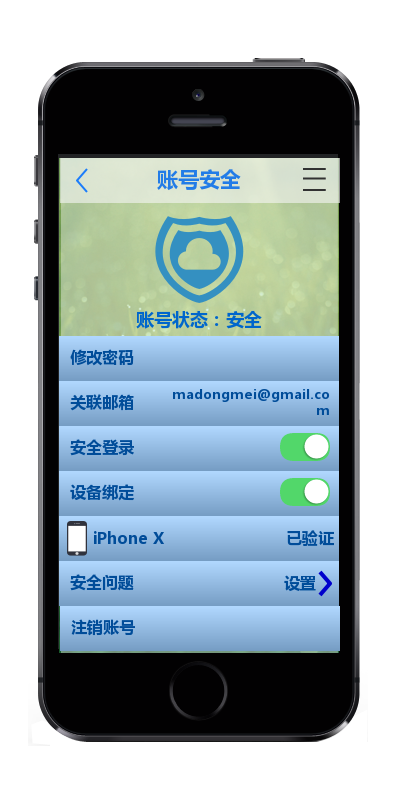
\includegraphics[scale=0.6]{OutlineDesign/figures/账号保护和隐私保护功能界面.png}
        \caption{账号保护和隐私保护功能界面}
        \label{fig:server_flow}
    \end{figure}
    \newpage
    %--------------------------------------------------------------------------
    \section{R.INTF.CALC.012: 日历管理功能界面}
    \begin{figure}[h]
        \centering
        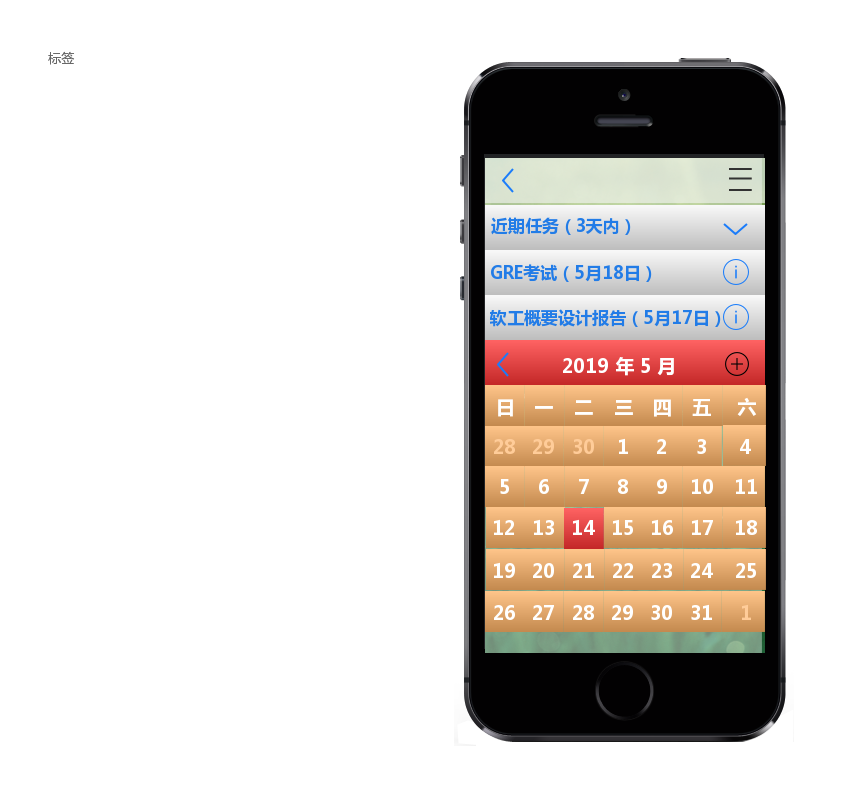
\includegraphics[scale=0.6]{OutlineDesign/figures/日历管理功能界面.png}
        \caption{日历管理功能界面}
        \label{fig:server_flow}
    \end{figure}
    \newpage
    %--------------------------------------------------------------------------
    \section{R.INTF.CALC.013: 个人本地和云端文件管理功能界面}
    \begin{figure}[h]
        \centering
        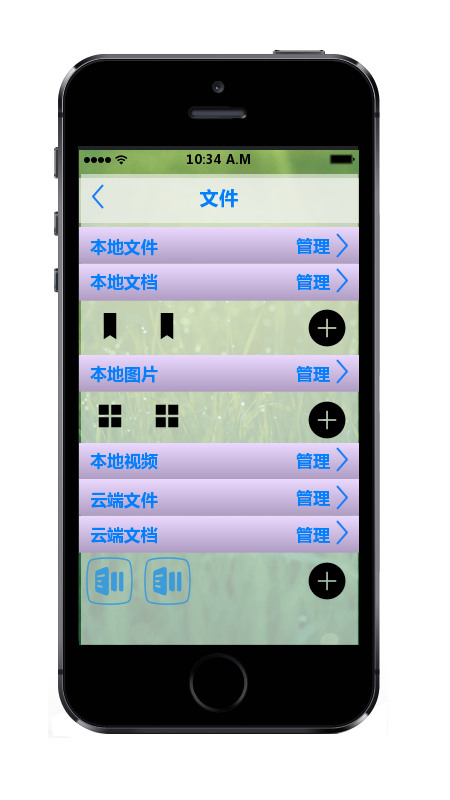
\includegraphics[scale=0.6]{OutlineDesign/figures/个人本地和云端文件管理功能界面.png}
        \caption{个人本地和云端文件管理功能界面}
        \label{fig:server_flow}
    \end{figure}
    \newpage
    %--------------------------------------------------------------------------
    \section{R.INTF.CALC.014: 邮箱接口功能界面}
    \begin{figure}[h]
        \centering
        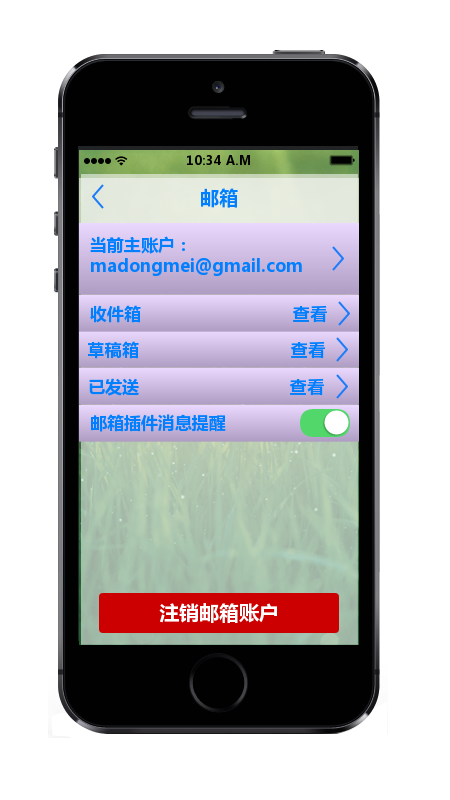
\includegraphics[scale=0.6]{OutlineDesign/figures/邮箱接口功能界面.png}
        \caption{邮箱接口功能界面}
        \label{fig:server_flow}
    \end{figure}
    \newpage
    %--------------------------------------------------------------------------
    \section{\color{red}R.INTF.CALC.015: 流程审批功能}
    \begin{figure}[h]
        \centering
        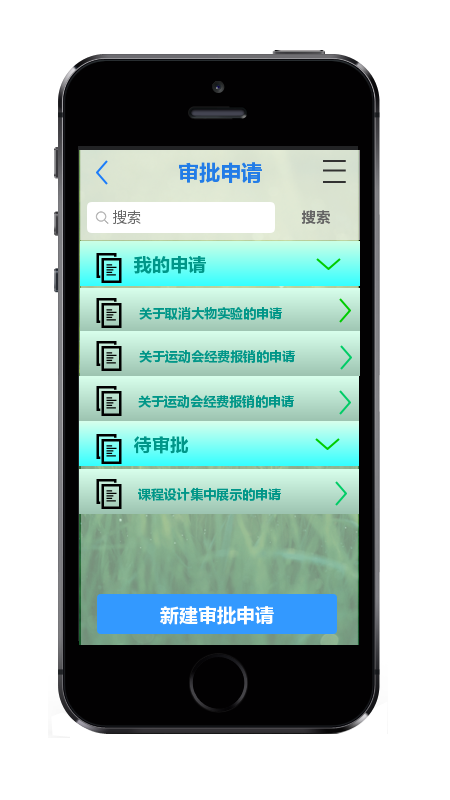
\includegraphics[scale=0.6]{OutlineDesign/figures/流程审批功能界面.png}
        \caption{\color{red}流程审批功能界面}
        \label{fig:server_flow}
    \end{figure}
    \newpage
    %--------------------------------------------------------------------------
    \section{\color{red}R.INTF.CALC.016: 信息调研功能}
    \begin{figure}[h]
        \centering
        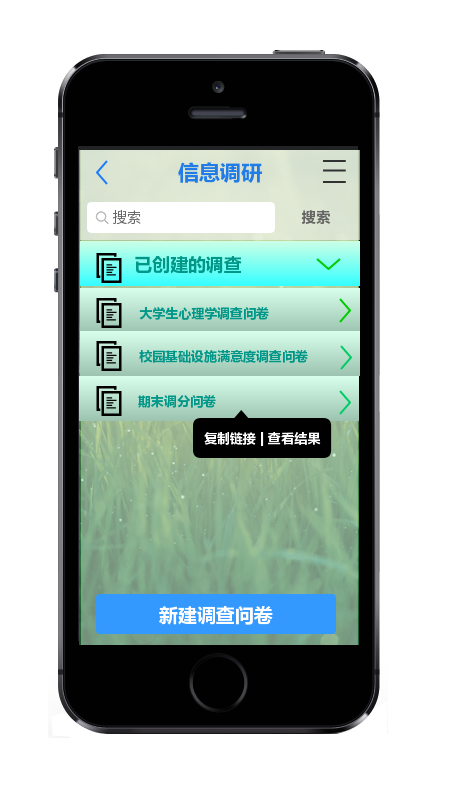
\includegraphics[scale=0.6]{OutlineDesign/figures/信息调研功能界面.png}
        \caption{\color{red}信息调研功能界面}
        \label{fig:server_flow}
    \end{figure}
    \newpage
    %--------------------------------------------------------------------------
    \section{\color{red}R.INTF.CALC.017: 第三方账号同步功能}
    \begin{figure}[h]
        \centering
        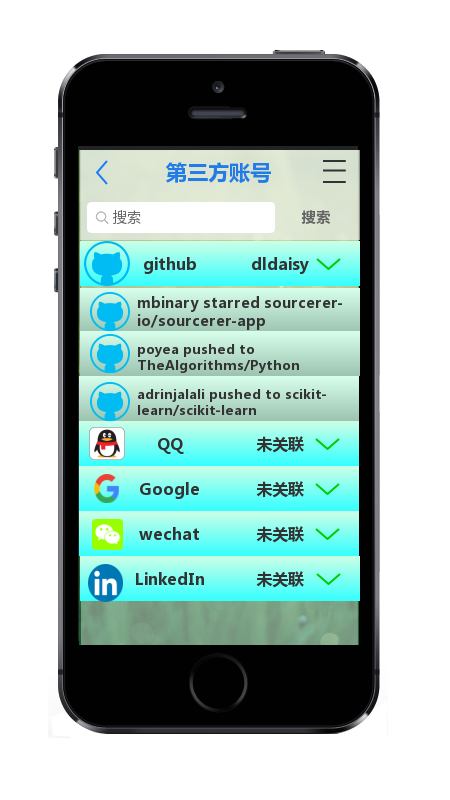
\includegraphics[scale=0.6]{OutlineDesign/figures/第三方账号同步功能界面.png}
        \caption{\color{red}第三方账号同步功能界面}
        \label{fig:server_flow}
    \end{figure}
    \newpage
    %--------------------------------------------------------------------------
    